% !TEX root = ../main.tex
%
% \section 建立表格与图片这一章，并自动更新后续章节编号以及目录中的页码。
\section{表格与图片：浮动体和交叉引用}

% learningbox 的花括号参数成为蓝色框标题；环境正文用于说明本章完成后应掌握的操作。
\begin{learningbox}{学习目标 / Learning goals}
学完本章后，你将能读写基本表格、制作三线表、按正文宽度缩放图片，
并用浮动体、标题、标签和交叉引用保持编号自动更新。
\end{learningbox}

% tabular 后的列格式决定列数和对齐方式；每行用 & 分隔单元格，用双反斜杠结束，二者数量要与列格式匹配。
\subsection{tabular 的行、列与对齐}

\texttt{tabular} 环境的列格式写在花括号中：\texttt{l} 表示左对齐，
\texttt{c} 表示居中，\texttt{r} 表示右对齐。每一行用 \verb|&| 分隔相邻单元格，
再用 \verb|\\| 结束当前行。比如列格式 \verb|{lcr}| 会依次建立左对齐、
居中和右对齐的三列；源码中每行也必须提供与这三列相匹配的内容。

% booktabs 提供粗细合适的 \toprule、\midrule、\bottomrule，三线表通常不再添加竖线。
\subsection{booktabs 三线表}

\texttt{booktabs} 宏包提供 \verb|\toprule|、\verb|\midrule| 和
\verb|\bottomrule|。下面的活动表格保留清晰的三线结构，并由 LaTeX 自动编号。

% table 的 [htbp] 给出候选位置；\centering 居中内容，\caption 生成编号后紧接 \label，标签才能保存正确的表号。
\begin{table}[htbp]
    \centering
    \caption{常用文档类型比较}
    \label{tab:document-types}
    \begin{tabular}{lcc}
        \toprule
        文档类型 & 适合内容 & 是否有 chapter \\
        \midrule
        article / ctexart & 短文、报告 & 否 \\
        book / ctexbook & 书籍、长文档 & 是 \\
        beamer & 幻灯片 & 不适用 \\
        \bottomrule
    \end{tabular}
\end{table}

% \includegraphics 的 width 选项控制图片宽度；用 0.82\textwidth 表示当前正文宽度的 82%，页面改变时会按比例缩放。
\subsection{插入和缩放图片}

\texttt{graphicx} 宏包提供 \verb|\includegraphics|。使用
\verb|width=0.82\textwidth|，可以让图片宽度保持为当前正文宽度的 82\%，
比写死厘米数更容易适应不同页面设置。

% figure 是浮动环境：图片命令负责插入文件，caption 负责图题和编号，label 保存编号供正文引用。
\begin{figure}[htbp]
    \centering
    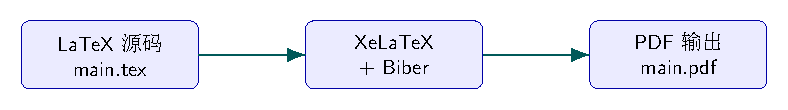
\includegraphics[width=0.82\textwidth]{figures/example-figure.pdf}
    \caption{从 LaTeX 源码到 PDF 的构建流程}
    \label{fig:build-flow}
\end{figure}

% 故意写错的图片路径位于 codeblock 中，只会显示为源码；若在正文执行，LaTeX 会因找不到文件而报错。
\begin{errorbox}
下面的命令指向一个不存在的文件；它只作为惰性源码显示，不会在本教程中执行：
\begin{codeblock}
\includegraphics{figures/missing-file.pdf}
\end{codeblock}
相对路径应从主文档的编译位置理解。本项目从 \texttt{main.tex} 所在目录编译，
所以 \texttt{figures/example-figure.pdf} 表示该目录下 \texttt{figures} 文件夹中的图片。
若文件名、扩展名、大小写或相对层级写错，LaTeX 就无法找到图片。
\end{errorbox}

% figure 和 table 后的 h、t、b、p 只是“此处附近、页顶、页底、浮动页”的候选位置，不是强制坐标。
\subsection{浮动体、标题与标签}

\texttt{figure} 和 \texttt{table} 都是浮动体。位置参数中的 \texttt{h} 建议放在当前位置附近，
\texttt{t} 建议放在页顶，\texttt{b} 建议放在页底，\texttt{p} 建议放到浮动体专页；
它们都是候选位置，不是把对象固定在某一点的绝对命令。LaTeX 会根据对象大小、页面余量
和浮动规则选择实际位置。

\verb|\caption| 生成图题或表题以及对应编号，\verb|\label| 保存这个编号。
通常把标签紧跟在标题之后，并用带类型前缀的名称区分图片和表格，例如
\texttt{fig:build-flow} 与 \texttt{tab:document-types}。

% \ref{标签名} 读取辅助文件中保存的编号；源码里的不换行空格 ~ 可避免“图”和编号被拆到两行。
\subsection{交叉引用}

使用 \verb|\ref| 可以读取标签所记录的编号。例如，
表~\ref{tab:document-types} 比较了三类常用文档，
图~\ref{fig:build-flow} 展示了从 \texttt{main.tex} 到 \texttt{main.pdf} 的构建流程。
加入或移动带标签的对象后需要再次编译，让辅助文件先写入编号、再把编号读回正文；
本项目的 LaTeXmk 会自动完成这些轮次。

% 章末 learningbox 汇总表格分隔符、浮动位置和交叉引用三类语法，内容仍按普通段落排版。
\begin{learningbox}{本章检查 / Chapter check}
我能解释 \texttt{l}、\texttt{c}、\texttt{r}、\verb|&| 和 \verb|\\| 的含义，
能区分浮动位置建议与固定位置，并能用 \verb|\label| 和 \verb|\ref| 自动维护图表编号。
\end{learningbox}
